\section{Compiling Matrix Operations to a Quantum Circuit}
In this section, we present our extended MLIR-based compilation pipeline, which enables the translation of matrix operations written in C directly into executable quantum circuits. We introduce our intermediate representations and discuss the design choices behind our implementation.

\subsection{Extended Compilation Pipeline}
% Figura pipeline
% Figura: Extended Pipeline Architecture
\begin{figure}[!htb]
\centering
\resizebox{0.85\columnwidth}{!}{%
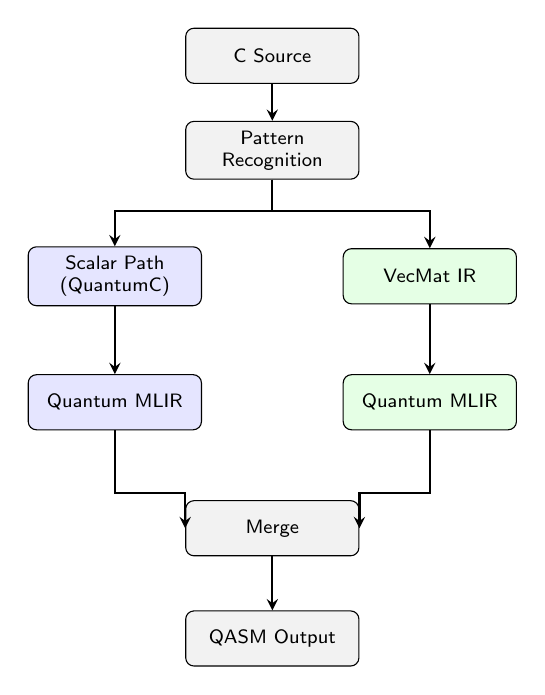
\begin{tikzpicture}[
    box/.style={
        draw,
        rounded corners=3pt,
        minimum width=2.2cm,
        minimum height=0.7cm,
        align=center,
        font=\sffamily\scriptsize
    },
    mainbox/.style={box, fill=gray!10},
    scalarbox/.style={box, fill=blue!10},
    vecbox/.style={box, fill=green!10},
    arrow/.style={->, >=stealth, thick}
]

% Riga 0: C Source
\node[mainbox] (source) at (0, 0) {C Source};

% Riga 1: Pattern Recognition
\node[mainbox] (pattern) at (0, -1.2) {Pattern\\Recognition};

% Riga 2: Branch - due path
\node[scalarbox] (scalar) at (-2, -2.8) {Scalar Path\\(QuantumC)};
\node[vecbox] (vecmat) at (2, -2.8) {VecMat IR};

% Riga 3: Entrambi producono Quantum MLIR
\node[scalarbox] (sqmlir) at (-2, -4.4) {Quantum MLIR};
\node[vecbox] (vqmlir) at (2, -4.4) {Quantum MLIR};

% Riga 4: Merge
\node[mainbox] (merge) at (0, -6.0) {Merge};

% Riga 5: QASM Output
\node[mainbox] (qasm) at (0, -7.4) {QASM Output};

% === FRECCE ===

% Top: source -> pattern
\draw[arrow] (source) -- (pattern);

% Branch: pattern -> scalar e pattern -> vecmat
\draw[arrow] (pattern.south) -- ++(0, -0.4) -| (scalar.north);
\draw[arrow] (pattern.south) -- ++(0, -0.4) -| (vecmat.north);

% Scalar path: scalar -> sqmlir
\draw[arrow] (scalar) -- (sqmlir);

% Vector path: vecmat -> vqmlir (lowering diretto)
\draw[arrow] (vecmat) -- (vqmlir);

% Convergenza verso Merge
\draw[arrow] (sqmlir.south) -- ++(0, -0.8) -| (merge.west);
\draw[arrow] (vqmlir.south) -- ++(0, -0.8) -| (merge.east);

% Bottom: merge -> qasm
\draw[arrow] (merge) -- (qasm);

\end{tikzpicture}%
}
\caption{Extended QuantumC compilation pipeline. The scalar path follows the original QuantumC stages, while the vector/matrix path processes recognized patterns through the VecMat IR with direct lowering to quantum operations.}
\label{fig:pipeline}
\end{figure}

\label{sec:compilation-pipeline}

These constraints are addressed by adopting Static Single Assignment (SSA) form, where each variable is assigned exactly once. Under this model, each variable in the source program is mapped to a dedicated quantum register, and each arithmetic operation becomes a quantum gate (or sequence of gates) that reads from input registers and writes to a fresh output register
QuantumC~\cite{quantumc} implements this approach using an MLIR-based compilation pipeline~\cite{mlir,xdsl}. The compiler parses C source code, generates an SSA-based intermediate representation, translates arithmetic and control-flow operations into quantum gates, and exports the circuit in OpenQASM~\cite{openqasm} format. However, the current implementation supports only scalar integer operations and does not handle arrays, vectors, or matrices---the gap that our extension addresses.
We extend the QuantumC pipeline with a dedicated path for vector and matrix operations, preserving compatibility with existing scalar compilation. Figure~\ref{fig:pipeline} illustrates the extended architecture. The following subsections detail the pipeline structure, intermediate representations, the pattern recognition and lowering process, and support for hybrid programs.
The original QuantumC pipeline processes C programs through five sequential stages, from AST generation to OpenQASM output. Our extension augments this pipeline with a dedicated compilation path for vector and matrix operations, while preserving full compatibility with the existing scalar infrastructure.

The compilation begins with a \emph{pattern recognition} phase that analyzes the C abstract syntax tree to identify vector and matrix computation patterns. When such patterns are detected, they are extracted from the AST and processed through a dedicated \emph{vector/matrix path}, while the remaining scalar code follows the standard QuantumC pipeline.

In the vector/matrix path, recognized patterns are represented in a high-level \emph{VecMat IR} that captures the semantic meaning of the computation. This intermediate representation is then lowered directly to quantum operations compatible with the existing QuantumC quantum dialect, allocating quantum registers for array elements and generating the appropriate arithmetic operations.

The two paths converge in a \emph{merge phase} that combines their quantum representations into a unified module. A \emph{result map} tracks the correspondence between high-level array elements and their quantum register assignments, ensuring that return statements and data dependencies are correctly resolved across the two paths.

\textbf{VecMat Intermediate Representation}
\label{sec:intermediate-repr}

\textcolor{red}{mergiare con quella prima }
To represent vector and matrix operations throughout the compilation process, we introduce a dedicated intermediate representation that integrates into the existing MLIR-based pipeline. The \emph{VecMat IR} captures vector and matrix operations at a high level of abstraction, preserving the semantic meaning of the computation without exposing implementation details.

The representation defines three core operations. \textbf{VecAdd} represents element-wise vector addition, capturing computations of the form $c[i] = a[i] + b[i]$ for $i = 0, \ldots, N-1$. \textbf{VecDot} represents dot product with scalar accumulation, corresponding to $s = \sum_{i=0}^{N-1} a[i] \cdot b[i]$. \textbf{MatMul} represents matrix multiplication $C = A \times B$, where $A$ is $M \times K$, $B$ is $K \times N$, and $C$ is $M \times N$.

Each operation records the names of input and output arrays, the relevant dimensions, and the element bitwidth. The VecMat IR also maintains a \emph{constant table} that stores compile-time initialization values extracted from C array initializers (e.g., \texttt{int a[4] = \{1,2,3,4\}}), along with their shapes. This information is essential for the subsequent lowering phase, which must initialize quantum registers with the correct values.

\begin{figure}[htb]
% Row 1: VecAdd and VecDot
\begin{minipage}{0.48\columnwidth}
\begin{lstlisting}[style=mlirstyle]
VecAdd {
  dest: "c"
  lhs: "a", rhs: "b"
  length: 4, elem_bits: 16
}
\end{lstlisting}
\centering\small (a) VecAdd
\end{minipage}
\hfill
\begin{minipage}{0.48\columnwidth}
\begin{lstlisting}[style=mlirstyle]
VecDot {
  dest: "s"
  lhs: "a", rhs: "b"
  length: 4, elem_bits: 16
}
\end{lstlisting}
\centering\small (b) VecDot
\end{minipage}

\vspace{0.5em}

% Row 2: MatMul (wider)
\begin{minipage}{\columnwidth}
\begin{lstlisting}[style=mlirstyle]
MatMul {
  dest: "C", lhs: "A", rhs: "B"
  m: 2, n: 2, k: 2, elem_bits: 16
}
\end{lstlisting}
\centering\small (c) MatMul
\end{minipage}
\caption{VecMat IR operations: vector addition, dot product, and matrix multiplication.}
\label{fig:ir-examples}
\end{figure}




\subsection{Hybrid Compilation}
\label{sec:hybrid}
\begin{figure*}[t]
\centering

% ----------------- COLORS -----------------
\definecolor{scalarcolor}{RGB}{66,133,244}
\definecolor{vectorcolor}{RGB}{52,168,83}
\definecolor{mergecolor}{RGB}{171,71,188}

% ----------------- STYLES -----------------
\tikzset{
  panelbox/.style={
    draw=gray!60,
    rounded corners=4pt,
    fill=gray!5,
    inner sep=6pt,
    minimum width=3.6cm
  },
  panellabel/.style={
    font=\sffamily\bfseries\small,
    fill=white,
    inner sep=2pt
  },
  flowarrow/.style={
    ->,
    >=stealth,
    line width=1pt,
    black
  }
}

\begin{tikzpicture}[node distance=0.4cm, every node/.style={align=left}]

% ================= PANEL (a) =================
\node[panelbox] (panelA) {
\begin{minipage}{3.4cm}
\begin{lstlisting}[basicstyle=\ttfamily\tiny, frame=none]
int main() {
  @\textcolor{scalarcolor}{int x = 5;}@
  @\textcolor{scalarcolor}{int y = 7;}@
  @\textcolor{scalarcolor}{int z = x + y;}@

  @\textcolor{vectorcolor}{int a[2] = {1, 2};}@
  @\textcolor{vectorcolor}{int b[2] = {3, 4};}@
  @\textcolor{vectorcolor}{int c[2];}@

  @\textcolor{vectorcolor}{for (int i = 0; i < 2;}@
       @\textcolor{vectorcolor}{i = i + 1) \{}@
    @\textcolor{vectorcolor}{c[i] = a[i]+b[i];}@
  @\textcolor{vectorcolor}{\}}@

  @\textcolor{mergecolor}{return z + c[0];}@
}
\end{lstlisting}
\end{minipage}
};
\node[panellabel, above=0pt of panelA.north] {(a) C Source};

% ================= PANEL (b) =================
\node[panelbox, right=0.6cm of panelA] (panelB) {
\begin{minipage}{3.4cm}
\textcolor{scalarcolor}{\scriptsize\sffamily\bfseries SCALAR PATH:}
\begin{lstlisting}[basicstyle=\ttfamily\tiny, frame=none]
int x = 5;
int y = 7;
int z = x + y;
return z + [ ];
\end{lstlisting}

\vspace{2pt}

\textcolor{vectorcolor}{\scriptsize\sffamily\bfseries VECTOR PATH:}
\begin{lstlisting}[basicstyle=\ttfamily\tiny, frame=none]
VecAdd {
  lhs: "a" = [1, 2]
  rhs: "b" = [3, 4]
  dest: "c", len: 2
}
\end{lstlisting}
\end{minipage}
};
\node[panellabel, above=0pt of panelB.north] {(b) Path Separation};

% ================= PANEL (c) =================
\node[panelbox, right=0.6cm of panelB] (panelC) {
\begin{minipage}{3.4cm}
\textcolor{scalarcolor}{\scriptsize\sffamily\bfseries SCALAR QUANTUM MLIR:}
\begin{lstlisting}[basicstyle=\ttfamily\tiny, frame=none]
%x = q.init 5
%y = q.init 7
%z = q.addi %x, %y
return %z
\end{lstlisting}

\vspace{2pt}

\textcolor{vectorcolor}{\scriptsize\sffamily\bfseries VECTOR QUANTUM OPS:}
\begin{lstlisting}[basicstyle=\ttfamily\tiny, frame=none]
%a0 = q.init 1
%a1 = q.init 2
%b0 = q.init 3
%b1 = q.init 4
%c0 = q.addi %a0, %b0
%c1 = q.addi %a1, %b1
\end{lstlisting}

\vspace{1pt}
{\tiny\sffamily result\_map: c[0] $\rightarrow$ \%c0}
\end{minipage}
};
\node[panellabel, above=0pt of panelC.north] {(c) Quantum IRs};

% ================= PANEL (d) =================
\node[panelbox, right=0.6cm of panelC] (panelD) {
\begin{minipage}{3.1cm}
\ttfamily\tiny
func @main() -> i32 \{\\
\textcolor{scalarcolor}{\%x = q.init 5}\\
\textcolor{scalarcolor}{\%y = q.init 7}\\
\textcolor{scalarcolor}{\%z = q.addi \%x, \%y}\\[2pt]

\textcolor{vectorcolor}{\%a0 = q.init 1}\\
\textcolor{vectorcolor}{\%a1 = q.init 2}\\
\textcolor{vectorcolor}{\%b0 = q.init 3}\\
\textcolor{vectorcolor}{\%b1 = q.init 4}\\
\textcolor{vectorcolor}{\%c0 = q.addi \%a0,\%b0}\\
\textcolor{vectorcolor}{\%c1 = q.addi \%a1,\%b1}\\[2pt]

\textcolor{mergecolor}{\%r = q.addi \%z, \%c0}\\
\textcolor{mergecolor}{return \%r}\\
\}
\end{minipage}
};
\node[panellabel, above=0pt of panelD.north] {(d) Merged Module};

% ================= ARROWS =================
\draw[flowarrow] (panelA.east) -- (panelB.west);
\draw[flowarrow] (panelB.east) -- (panelC.west);
\draw[flowarrow] (panelC.east) -- (panelD.west);

% ================= LEGEND =================
\node at ($(panelA.south west)+(0,-0.7cm)$) [anchor=north west] {
    \scriptsize\sffamily
    \textcolor{scalarcolor}{$\blacksquare$} Scalar path \quad
    \textcolor{vectorcolor}{$\blacksquare$} Vector path \quad
    \textcolor{mergecolor}{$\blacksquare$} Merge point
};

\end{tikzpicture}

\caption{Hybrid compilation: a C program containing both scalar and vector operations is split into two compilation paths. The scalar path follows the standard QuantumC pipeline, while the vector path is processed through the VecMat IR. Both paths are merged into a unified quantum module, with the \emph{result\_map} resolving array element references (e.g., \texttt{c[0]} $\rightarrow$ \texttt{\%c0}).}
\label{fig:hybrid-compilation}

\end{figure*}

Programs may contain both scalar arithmetic and vector/matrix operations. The extended pipeline handles these \emph{hybrid programs} by processing each component through the most appropriate path and then combining the results into a unified quantum module. Figure~\ref{fig:hybrid-compilation} illustrates this process with a concrete example.

% Figura: Hybrid Compilation (path separation and merge)


\textbf{Path Separation.} During pattern recognition, loops that match vector or matrix patterns are extracted from the AST and processed through the vector/matrix path. The remaining code---including scalar variable declarations, arithmetic operations, control flow constructs, and return statements---is processed through the standard QuantumC scalar path. This separation ensures that each component is compiled using the most efficient representation.

\textbf{Merge Phase.} After both paths have generated their respective quantum representations, a merge phase combines them into a single quantum module. The merge operates on the scalar module, inserting operations from the vector/matrix module at appropriate locations.

The operations from the vector/matrix path are divided into two categories: \emph{initialization operations} (\texttt{quantum.init}) that allocate and initialize quantum registers, and \emph{arithmetic operations} (\texttt{quantum.addi}, \texttt{quantum.muli}) that perform computations. Initialization operations are inserted at the beginning of the function, grouped with the scalar path's initializations. Arithmetic operations are inserted immediately before the return statement, ensuring that all computations complete before the function returns.

During insertion, SSA values must be remapped: when an operation is cloned from the vector/matrix module into the scalar module, its operands must be updated to reference the cloned registers rather than the original ones. An \emph{SSA map} tracks the correspondence between original and cloned values throughout the merge process.

\textbf{Return Value Resolution.} A key challenge arises when the original C program's return statement references array elements computed by the vector/matrix path. In the simplest case, such as \texttt{return c[2]} for a vector or \texttt{return C[1][0]} for a matrix, the scalar path has no knowledge of the array and generates a placeholder return value initialized to zero. During the merge phase, the compiler detects this placeholder and replaces it with the correct quantum register from the \emph{result map}.

A more complex situation occurs when the return statement combines scalar and array values, as shown in Figure~\ref{fig:hybrid-compilation} with \texttt{return z + c[0]}. Here, the scalar path correctly computes the scalar operand \texttt{z}, but cannot access the array element computed by the vector path. In this case, the compiler extracts a \emph{hybrid return hint} that records both the arithmetic operation and the array element reference. During merge, since the scalar return value is not a placeholder, the compiler emits a new quantum operation to combine the scalar result with the array element looked up from the result map.

To enable this resolution, the compiler extracts \emph{return hints} from the original C AST before path separation. These hints record which array elements, and any associated arithmetic operations, appear in return statements, allowing the merge phase to correctly connect quantum registers across the two compilation paths.


\subsection{Pattern Recognition and Lowering}
\label{sec:pattern-lowering}


The pattern recognition phase identifies common vector and matrix computations by analyzing the structure of loop constructs in the C abstract syntax tree. Rather than relying on explicit annotations or library calls, our approach recognizes computation patterns based on their syntactic structure, enabling the compiler to capture high-level semantics that would otherwise be lost through naive loop unrolling.

The recognition algorithm traverses the AST and examines each \texttt{for} loop, checking whether its structure matches one of the supported patterns. For a loop to be recognized, it must satisfy several conditions: (1)~the loop header must follow a canonical form with initialization to zero, a comparison against a constant bound, and unit increment; (2)~the loop body must contain array accesses indexed by the loop variable; and (3)~the computation must match the expected arithmetic structure.

Table~\ref{tab:patterns} summarizes the three supported patterns. \emph{Vector addition} is recognized as a single loop where each iteration computes \texttt{c[i] = a[i] + b[i]}. \emph{Dot product} is identified by a single loop with scalar accumulation of the form \texttt{s = s + a[i] * b[i]}. \emph{Matrix multiplication} requires a triple nested loop structure with indices \texttt{i}, \texttt{j}, \texttt{k}, where the innermost computation accumulates products of the form \texttt{A[i][k] * B[k][j]} into the result matrix \texttt{C[i][j]}.

When a pattern is successfully matched, the corresponding loop is removed from the AST that will be processed by the scalar path, and a high-level operation is created in the VecMat IR. Loops that do not match any pattern remain in the AST and are processed through the standard QuantumC pipeline with static unrolling.

\begin{table}[!htb]
  \caption{Supported Vector and Matrix Patterns}
  \label{tab:patterns}
  \centering
  \small
  \setlength{\tabcolsep}{6pt}
  \begin{tabularx}{\linewidth}{l>{\ttfamily\raggedright\arraybackslash}X l}
    \toprule
    Pattern & C Code Structure & Loop Nesting \\
    \midrule
    Vector addition & c[i] = a[i] + b[i] & Single loop \\
    Dot product & s = s + a[i] * b[i] & Single loop \\
    Matrix multiplication & C[i][j] += A[i][k] * B[k][j] & Triple nested \\
    \bottomrule
  \end{tabularx}
\end{table}

\noindent\textbf{Lowering to Quantum Operations.}
\label{sec:arith_matrix}

The lowering phase translates high-level VecMat operations into sequences of quantum arithmetic primitives. The key insight is that matrix multiplication decomposes naturally into multiply-accumulate (MAC) operations: computing each element $C[i][j] = \sum_{k=0}^{n-1} A[i][k] \cdot B[k][j]$ requires $n$ multiplications followed by $n$ additions to accumulate the partial products. Figure~\ref{fig:matmul-circuits} illustrates this decomposition and shows how the same MAC operation is implemented using the two arithmetic backends supported by our compiler.

% Figura matmul circuits
% Figura: Matrix Multiplication Quantum Circuits
% Mostra la struttura riga × colonna completa per un elemento

\begin{figure*}[t]
\centering

% Parte superiore: Visualizzazione riga × colonna
\begin{tikzpicture}[
    cell/.style={draw, minimum size=7mm, anchor=center},
    hlcell/.style={cell, fill=blue!20},
    matlabel/.style={font=\bfseries}
]

% Matrice A
\node[hlcell] (a00) at (0,0) {$a_{00}$};
\node[hlcell, right=-\pgflinewidth of a00] (a01) {$a_{01}$};
\node[cell, below=-\pgflinewidth of a00] (a10) {$a_{10}$};
\node[cell, right=-\pgflinewidth of a10] (a11) {$a_{11}$};
\node[matlabel, above=2mm of a00.north east] {$A$};

% Simbolo ×
\node[right=6mm of a01, font=\Large] (times) {$\times$};

% Matrice B
\node[cell, right=12mm of a01] (b00) {$b_{00}$};
\node[hlcell, right=-\pgflinewidth of b00] (b01) {$b_{01}$};
\node[cell, below=-\pgflinewidth of b00] (b10) {$b_{10}$};
\node[hlcell, right=-\pgflinewidth of b10] (b11) {$b_{11}$};
\node[matlabel, above=2mm of b00.north east] {$B$};

% Simbolo =
\node[right=6mm of b01, font=\Large] (eq) {$=$};

% Matrice C
\node[cell, right=12mm of b01] (c00) {$c_{00}$};
\node[hlcell, right=-\pgflinewidth of c00] (c01) {$c_{01}$};
\node[cell, below=-\pgflinewidth of c00] (c10) {$c_{10}$};
\node[cell, right=-\pgflinewidth of c10] (c11) {$c_{11}$};
\node[matlabel, above=2mm of c00.north east] {$C$};

% Formula esplicita
\node[right=10mm of c01, align=left, font=\small] {
    $c_{01} = a_{00} \cdot b_{01} + a_{01} \cdot b_{11}$\\[2pt]
    \textit{(row 0 $\times$ column 1)}
};

\end{tikzpicture}

\vspace{0.6em}

{\small $\downarrow$ \textit{quantum circuit for computing $c_{01}$}}

\vspace{0.4em}

% Circuito QFT completo
\textbf{(a) QFT-based backend}
\vspace{0.3em}

\begin{tikzpicture}
\begin{yquant*}
    qubit {$\ket{a_{00}}$} a00;
    qubit {$\ket{b_{01}}$} b01;
    qubit {$\ket{a_{01}}$} a01;
    qubit {$\ket{b_{11}}$} b11;
    qubit {$\ket{0}$} acc;

    % MAC #1: a00 × b01 → acc (QFT multiplication + QFT addition)
    box {QFT} acc;
    box {$CC\text{-}R_\phi$} (a00, b01, acc);
    box {$R_\phi$} acc;
    box {IQFT} acc;

    % MAC #2: a01 × b11 → acc
    box {QFT} acc;
    box {$CC\text{-}R_\phi$} (a01, b11, acc);
    box {$R_\phi$} acc;
    box {IQFT} acc;

    output {$\ket{a_{00}}$} a00;
    output {$\ket{b_{01}}$} b01;
    output {$\ket{a_{01}}$} a01;
    output {$\ket{b_{11}}$} b11;
    output {$\ket{c_{01}}$} acc;
\end{yquant*}
\end{tikzpicture}

{\footnotesize Multiplication via controlled-controlled phase rotations ($CC\text{-}R_\phi$); addition via controlled phase rotations ($R_\phi$).}

\vspace{0.5em}

% Circuito Ripple-carry completo
\textbf{(b) Ripple-carry backend}
\vspace{0.3em}

\begin{tikzpicture}
\begin{yquant*}
    qubit {$\ket{a_{00}}$} a00;
    qubit {$\ket{b_{01}}$} b01;
    qubit {$\ket{a_{01}}$} a01;
    qubit {$\ket{b_{11}}$} b11;
    qubit {$\ket{0}$} acc;
    qubit {$\ket{0}$} anc;

    % MAC #1: a00 × b01 → acc (shift-and-add multiplication + ripple addition)
    box {shift} (a00, acc);
    box {C-ADD} (b01, acc, anc);
    box {MAJ} (acc, anc);
    box {$\cdots$} (acc, anc);
    box {UMA} (acc, anc);

    % MAC #2: a01 × b11 → acc
    box {shift} (a01, acc);
    box {C-ADD} (b11, acc, anc);
    box {MAJ} (acc, anc);
    box {$\cdots$} (acc, anc);
    box {UMA} (acc, anc);

    output {$\ket{a_{00}}$} a00;
    output {$\ket{b_{01}}$} b01;
    output {$\ket{a_{01}}$} a01;
    output {$\ket{b_{11}}$} b11;
    output {$\ket{c_{01}}$} acc;
    output {$\ket{0}$} anc;
\end{yquant*}
\end{tikzpicture}

{\footnotesize Multiplication via shift-and-add with controlled ripple addition (C-ADD); addition via majority (MAJ) and unmajority (UMA) gates.}

\vspace{0.4em}
{\small $\vdots$ \textit{repeated for each element $c_{ij}$ using row $i$ of $A$ and column $j$ of $B$}}

\caption{Quantum circuits for matrix multiplication. To compute element $c_{01}$, the circuit performs two multiply-accumulate (MAC) operations using row~0 of $A$ ($a_{00}, a_{01}$) and column~1 of $B$ ($b_{01}, b_{11}$). The two backends differ in both multiplication and addition: (a)~QFT-based uses controlled-controlled phase rotations for multiplication and controlled phase rotations for addition, all operating in the Fourier basis; (b)~Ripple-carry uses shift-and-add for multiplication and Cuccaro's majority/unmajority gates for addition, requiring ancilla qubits. This structure repeats for each output element $c_{ij}$.}
\label{fig:matmul-circuits}
\end{figure*}


\textbf{Quantum Arithmetic Primitives.}
\label{sec:quantum-arithmetic}
Quantum arithmetic subroutines are essential building blocks in many quantum algorithms. In Grover's search~\cite{grover}, arithmetic comparators are used within oracles to mark target states satisfying numerical conditions. Shor's factoring algorithm~\cite{shor} relies on modular exponentiation, which decomposes into sequences of modular additions and multiplications. The HHL algorithm~\cite{hhl} for solving linear systems uses arithmetic operations to manipulate eigenvalues during matrix inversion. More broadly, any quantum algorithm that processes classical data encoded in quantum registers requires arithmetic primitives to manipulate those values.

Addition is the most basic arithmetic operation, and two main approaches exist for its quantum implementation.

\textbf{QFT-based addition.} The approach introduced by Draper~\cite{draper-qft} performs addition in the Fourier basis. The target register is first transformed via the Quantum Fourier Transform (QFT), then the addend is incorporated through controlled phase rotations, and finally the inverse QFT is applied to return to the computational basis. This method does not require ancilla qubits for carry propagation, as the carry information is encoded in the phase of the quantum state.

\textbf{Ripple-carry addition.} The approach proposed by Cuccaro et al.~\cite{cuccaro-ripple} follows the classical model of carry propagation. It uses a sequence of majority and unmajority gates, implemented with Toffoli (CCX) and CNOT gates, to propagate the carry bit through the register. This method requires ancilla qubits to store intermediate carry values but operates entirely in the computational basis without requiring the QFT.

To illustrate, adding $2 + 3$ with 3-qubit registers involves encoding the operands as $|010\rangle$ and $|011\rangle$. The addition circuit---whether QFT-based or ripple-carry---transforms these inputs and produces $|101\rangle$ (decimal 5) in the output register, while preserving the original operands for reversibility.

Other arithmetic operations in our compilation flow are built upon addition. Subtraction is performed via two's complement negation followed by addition. Multiplication can be implemented through repeated additions (shift-and-add) or using QFT-based techniques with controlled-controlled phase rotations.

The two addition approaches present different trade-offs in terms of qubit count, circuit depth, and gate composition. These trade-offs depend on the target hardware characteristics, such as native gate sets and qubit connectivity. Our extended compiler supports both backends, and we present a comparative analysis in Section~\ref{sec:results}.
The final stage of the vector/matrix path translates VecMat IR operations directly into quantum operations compatible with the QuantumC quantum dialect. This lowering phase performs two key tasks: allocating and initializing quantum registers for array elements, and generating the arithmetic operations that implement the computation.

Each array element is mapped to a dedicated quantum register. For a vector of length $N$, the lowering allocates $N$ registers; for an $M \times N$ matrix, it allocates $M \times N$ registers in row-major order. When compile-time initialization values are available from the constant table, registers are initialized to the corresponding values using \texttt{quantum.init} operations.

The lowering of VecMat operations proceeds as follows. For VecAdd, the lowering generates $N$ independent \texttt{quantum.addi} operations, each adding corresponding elements from the input vectors. For VecDot, a sequence of multiply-accumulate operations is generated: for each index $i$, a \texttt{quantum.muli} computes $a[i] \cdot b[i]$, followed by \texttt{quantum.addi} to accumulate the result into a scalar register. For MatMul, each element $C[i][j]$ requires $K$ multiply-accumulate operations to compute the inner product $\sum_{k=0}^{K-1} A[i][k] \cdot B[k][j]$.

During lowering, a \emph{result map} is constructed that associates each array element with its final quantum register. This mapping is essential for the merge phase, which must connect the correct quantum register to return statements that reference array elements.

